% Provenance (never printed): cycle 4 SVT, "La planete Terre": the history of
% the Earth read in the rocks, relative dating (superposition, recoupement,
% inclusion, continuite paleontologique), the ages of the Earth, eras and
% periods, the scale of geological time; see sources/book1/PROVENANCE.md.
% Book 1, grade 7, chapter 5.
% Vocabulary guard: owns relative dating / absolute age, the four principles,
% unconformity, era and geological period, the geological time scale. The
% method of radiometric dating is the physics books' and grade 12's: told
% here in two sentences, never defined. Fossils as evidence of evolution are
% the biology books' (one sentence of prose). "Ice age" is grade 8's: not used.
\chapter{The Ages of the Earth}\label{ch:g7:geological-time}

In June 1788, the Scottish geologist James Hutton and two friends, the
mathematician John Playfair and the chemist James Hall, visited Siccar
Point, a rocky point ``washed bare by the \omterm{def:g2:water-on-earth:ocean}{sea}'' on the \omterm{def:g1:landscapes-around-us:water}{coast} of Scotland.
At the bottom of the \omterm{def:g3:stones-pebbles-sand:rock}{rock} they saw grey layers standing on end, almost
vertical. Above them lay layers of red sandstone, gently sloping. Hutton
explained what had happened: the grey layers had been laid down flat on
the floor of a \omterm{def:g2:water-on-earth:ocean}{sea}, then pushed up on end, then worn away, before the red
\omterm{def:g3:stones-pebbles-sand:sand}{sand} was laid on top of them. Each of these steps needed an immense
time. Playfair wrote later: ``The mind seemed to grow giddy by looking so
far into the abyss of time.''
% ledger: ncse:siccar-point

\begin{omfigure}
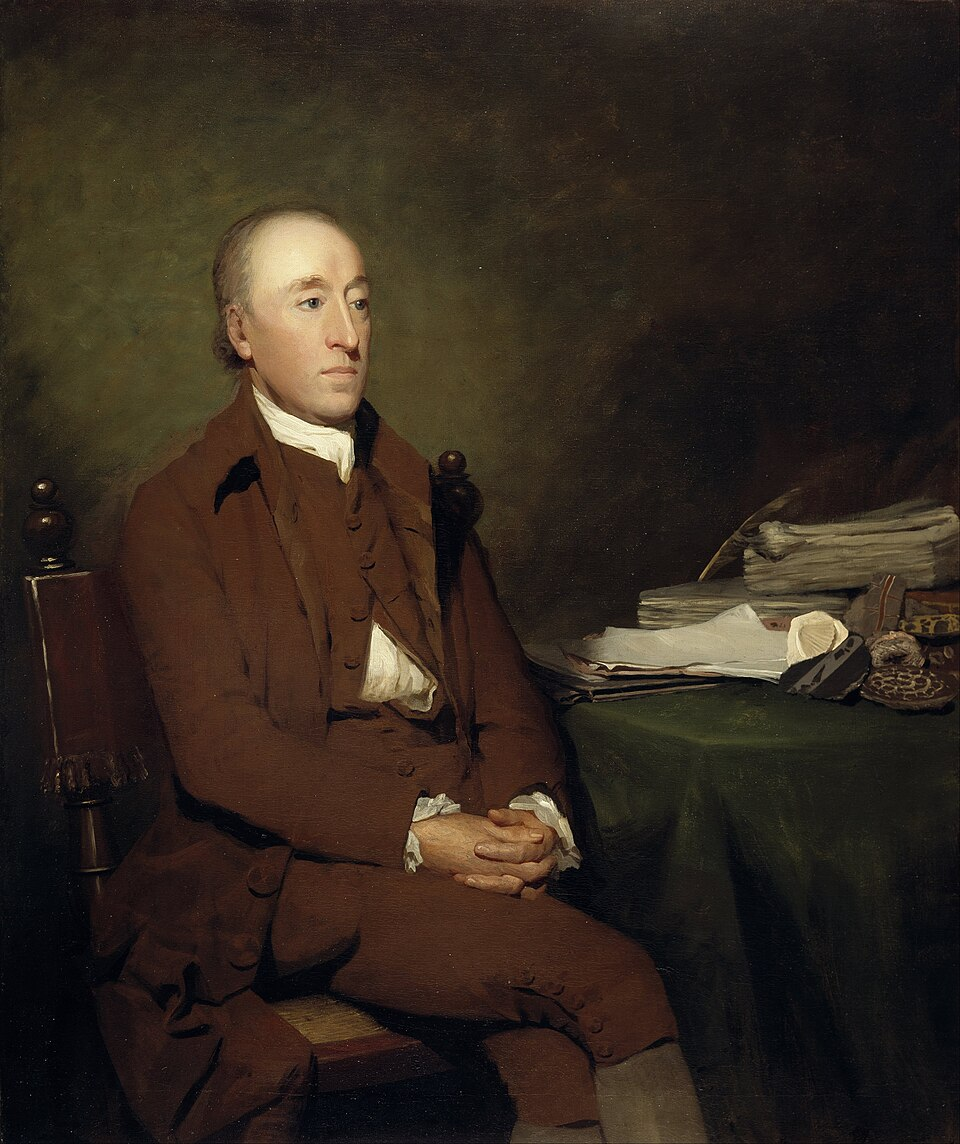
\includegraphics[width=0.3\linewidth]{images/book1/g7-hutton.jpg}

{\small James Hutton (1726--1797), painted by Henry Raeburn. Hutton
saw each layer as a span of time, with the oldest at the bottom
wherever the layers have not been turned over. Portrait in the public domain, via Wikimedia
Commons.}
% ledger: commons:hutton-portrait, usgs:hutton-smith
\label{fig:g7:geological-time:hutton}
\end{omfigure}

How can we tell which \omterm{def:g3:stones-pebbles-sand:rock}{rock} is older than another, without any date
written on it? How old is the Earth? And how can such a long history be
pictured at all?

\begin{recall}
\omterm{def:g7:sediments-and-fossils:sediment}{Sediments} settle in layers, one on top of the other, and harden into
\omterm{def:g6:rocks-and-minerals:rock-families}{sedimentary rock}; \omterm{def:g7:sediments-and-fossils:fossil}{fossils} are the remains or traces of living things
kept in \omterm{def:g3:stones-pebbles-sand:rock}{rock} (\cref{ch:g7:sediments-and-fossils}). A \emph{\omterm{def:g7:earthquakes:fault}{fault}} is a
break in the \omterm{def:g3:stones-pebbles-sand:rock}{rocks} along which the two sides have moved
(\cref{ch:g7:earthquakes}). Granite is an \emph{\omterm{def:g6:rocks-and-minerals:rock-families}{igneous rock}}: it forms
when molten \omterm{def:g3:stones-pebbles-sand:rock}{rock} cools slowly, deep underground; schist is a
\emph{\omterm{def:g6:rocks-and-minerals:rock-families}{metamorphic rock}}, changed by heat and pressure; a conglomerate is
a \omterm{def:g6:rocks-and-minerals:rock-families}{sedimentary rock} made of \omterm{def:g3:stones-pebbles-sand:pebble}{pebbles} cemented together
(\cref{ch:g6:rocks-and-minerals}).
\end{recall}

\section{Which came first?}

Historians can put events in order even without their dates. The First
World War came before the Second: their names say so. Television was not
yet in homes when the Wright brothers first flew in 1903, but many
people watched the first steps on the Moon on television in 1969: so the
flight came first, then television in homes, then the Moon. Gathering
clues and comparing them is enough to find the order. For almost all of
the Earth's history there is no written record at all, and geologists
work the same way: they use clues kept in the \omterm{def:g3:stones-pebbles-sand:rock}{rocks}.
% ledger: usgs:events-order

\begin{definition}[Relative dating and absolute age]\label{def:g7:geological-time:relative-dating}
\emph{Relative dating}\index{relative dating} puts \omterm{def:g3:stones-pebbles-sand:rock}{rocks} and events in
order, from the oldest to the youngest, without saying how many years
ago they happened: this \omterm{def:g3:stones-pebbles-sand:rock}{rock} is older than that one. An \emph{absolute
age}\index{absolute age} is an age given as a number of years, for
example ``\num{300} million years''.
\end{definition}

\section{Four principles for putting rocks in order}

Four simple principles do most of the work of \omterm{def:g7:geological-time:relative-dating}{relative dating}. They are
pictured below, in four imagined cliffs. The first was stated by Nicolas Steno in 1669; Hutton built on it at the end of the eighteenth century.
% ledger: usgs:hutton-smith, og:stratigraphy-principles

\begin{omfigure}
\tikzset{
  trilo/.pic={\fill[black!65] (0,0) ellipse (0.13 and 0.085);
              \draw[white, line width=0.3pt] (-0.11,0.028) -- (0.11,0.028) (-0.11,-0.028) -- (0.11,-0.028);},
  ammo/.pic={\draw[black!75, line width=0.45pt] (0,0) circle (0.1) (0,0) circle (0.062) (0,0) circle (0.028);}
}
\begin{minipage}[t]{0.49\linewidth}\centering
\begin{tikzpicture}[font=\footnotesize]
  \fill[lith sandstone] (0,0) rectangle (4.4,0.6);
  \fill[lith shale] (0,0.6) rectangle (4.4,1.2);
  \fill[lith limestone] (0,1.2) rectangle (4.4,1.8);
  \fill[lith sandstone] (0,1.8) rectangle (4.4,2.4);
  \foreach \k in {1,2,3,4} \node[fill=white, inner sep=1pt] at (0.35,0.6*\k-0.3) {\k};
  \draw (0,0) rectangle (4.4,2.4);
  \foreach \y in {0.6,1.2,1.8} \draw[contact] (0,\y) -- (4.4,\y);
  \draw[-{Stealth}, line width=0.8pt] (4.75,0.1) -- (4.75,2.3);
  \node[anchor=west] at (4.85,2.2) {youngest};
  \node[anchor=west] at (4.85,0.2) {oldest};
\end{tikzpicture}

{\small (a) Superposition: layer 1 formed first, layer 4 last.}
\end{minipage}\hfill
\begin{minipage}[t]{0.49\linewidth}\centering
\begin{tikzpicture}[font=\footnotesize]
  % left block, below the fault
  \begin{scope}
    \clip (0,0) -- (3.75,0) -- (3.25,2.4) -- (0,2.4) -- cycle;
    \fill[lith sandstone] (0,0) rectangle (5,0.6);
    \fill[lith shale] (0,0.6) rectangle (5,1.2);
    \fill[lith limestone] (0,1.2) rectangle (5,1.8);
    \fill[lith granite] (1.2,0) -- (1.85,0) -- (1.75,0.9) -- (1.9,1.8) -- (1.15,1.8) -- (1.3,0.9) -- cycle;
    \fill[lith sandstone] (0,1.8) rectangle (5,2.4);
    \foreach \y in {0.6,1.2} {\draw[contact] (0,\y) -- (1.25,\y); \draw[contact] (1.8,\y) -- (5,\y);}
    \draw[contact] (1.2,0) -- (1.3,0.9) -- (1.15,1.8) (1.85,0) -- (1.75,0.9) -- (1.9,1.8);
    \draw[contact] (0,1.8) -- (5,1.8);
  \end{scope}
  % right block, moved down along the fault
  \begin{scope}
    \clip (3.75,0) -- (5,0) -- (5,2.05) -- (3.32,2.05) -- cycle;
    \fill[lith sandstone] (3,-0.35) rectangle (5,0.25);
    \fill[lith shale] (3,0.25) rectangle (5,0.85);
    \fill[lith limestone] (3,0.85) rectangle (5,1.45);
    \fill[lith sandstone] (3,1.45) rectangle (5,2.05);
    \foreach \y in {0.25,0.85,1.45} \draw[contact] (3,\y) -- (5,\y);
  \end{scope}
  \draw (0,0) -- (5,0) -- (5,2.05) -- (3.32,2.05) (3.25,2.4) -- (0,2.4) -- (0,0);
  \draw[fault] (3.75,0) -- (3.25,2.4);
  \node[anchor=south, fill=white, inner sep=1pt] at (1.5,2.45) {granite};
  \draw[black!70] (1.5,2.45) -- (1.52,1.6);
  \node[anchor=south] at (4.2,2.45) {fault};
  \draw[black!70] (4.0,2.45) -- (3.4,1.75);
\end{tikzpicture}

{\small (b) Cross-cutting: the granite is younger than the three layers
it cuts, older than the top layer; the \omterm{def:g7:earthquakes:fault}{fault}, which breaks them all, is
the youngest.}
\end{minipage}

\bigskip
\begin{minipage}[t]{0.49\linewidth}\centering
\begin{tikzpicture}[font=\footnotesize]
  \fill[lith granite] (0,0) -- (4.4,0) -- (4.4,1.05) .. controls (3.4,0.95) and (2.6,1.2) .. (1.6,1.0) .. controls (0.9,0.88) and (0.4,1.1) .. (0,1.0) -- cycle;
  \fill[lith conglomerate] (0,2.4) -- (4.4,2.4) -- (4.4,1.05) .. controls (3.4,0.95) and (2.6,1.2) .. (1.6,1.0) .. controls (0.9,0.88) and (0.4,1.1) .. (0,1.0) -- cycle;
  \foreach \x/\y/\a/\b in {0.5/1.35/0.2/0.12, 1.3/1.25/0.16/0.1, 2.1/1.45/0.22/0.13, 2.9/1.3/0.17/0.11, 3.7/1.4/0.2/0.12, 0.9/1.8/0.15/0.1, 2.5/1.95/0.17/0.1, 3.4/1.85/0.14/0.09}
    \filldraw[fill=omLithGranite, draw=black!70, line width=0.3pt] (\x,\y) ellipse [x radius=\a, y radius=\b];
  \draw[unconformity] (0,1.0) .. controls (0.4,1.1) and (0.9,0.88) .. (1.6,1.0) .. controls (2.6,1.2) and (3.4,0.95) .. (4.4,1.05);
  \draw (0,0) rectangle (4.4,2.4);
  \node[fill=white, inner sep=1pt] at (2.2,0.45) {granite};
  \node[anchor=west] at (4.5,1.7) {conglomerate};
  \node[anchor=west, align=left] at (4.5,1.15) {pebbles of\\granite};
  \draw[black!70] (4.5,1.15) -- (3.85,1.4);
\end{tikzpicture}

{\small (c) Inclusion: the \omterm{def:g3:stones-pebbles-sand:pebble}{pebbles} of granite are older than the
conglomerate that holds them.}
\end{minipage}\hfill
\begin{minipage}[t]{0.49\linewidth}\centering
\begin{tikzpicture}[font=\footnotesize]
  % place A
  \fill[lith shale] (0,0) rectangle (1.3,0.8);
  \fill[lith limestone] (0,0.8) rectangle (1.3,1.6);
  \fill[lith sandstone] (0,1.6) rectangle (1.3,2.4);
  \draw (0,0) rectangle (1.3,2.4); \draw[contact] (0,0.8) -- (1.3,0.8) (0,1.6) -- (1.3,1.6);
  \foreach \x in {0.3,0.65,1.0} {\pic at (\x,0.4) {trilo}; \pic at (\x,1.2) {ammo};}
  \node[anchor=south] at (0.65,2.45) {place A};
  % place B
  \fill[lith sandstone] (3.6,0.4) rectangle (4.9,1.0);
  \fill[lith shale] (3.6,1.0) rectangle (4.9,2.0);
  \fill[lith limestone] (3.6,0) rectangle (4.9,0.4);
  \draw (3.6,0) rectangle (4.9,2.0); \draw[contact] (3.6,0.4) -- (4.9,0.4) (3.6,1.0) -- (4.9,1.0);
  \foreach \x in {3.9,4.25,4.6} {\pic at (\x,0.7) {trilo}; \pic at (\x,1.5) {ammo};}
  \node[anchor=south] at (4.25,2.45) {place B};
  \draw[dashed, black!70] (1.3,0.8) -- (3.6,1.0) (1.3,0) -- (3.6,0.4) (1.3,1.6) -- (3.6,2.0);
  \pic at (2.15,-0.3) {trilo}; \node[anchor=west] at (2.3,-0.3) {trilobite};
  \pic at (2.15,2.3) {ammo}; \node[anchor=west] at (2.3,2.3) {ammonite};
\end{tikzpicture}

{\small (d) \omterm{def:g7:sediments-and-fossils:fossil}{Fossil} succession: the layers with the same \omterm{def:g7:sediments-and-fossils:fossil}{fossils} are of
the same age, although their \omterm{def:g3:stones-pebbles-sand:rock}{rocks} differ.}
\end{minipage}

\medskip
{\small The four principles of \omterm{def:g7:geological-time:relative-dating}{relative dating}, in four imagined
cliffs.}
% ledger: usgs:hutton-smith, usgs:cross-cutting, nps:cross-cutting, eli:relative-dating, usgs:fossil-succession
\label{fig:g7:geological-time:principles}
\end{omfigure}

\begin{definition}[Principle of superposition]\label{def:g7:geological-time:superposition}
The \emph{principle of superposition}\index{superposition, principle of}:
in a pile of \omterm{def:g7:sediments-and-fossils:layer}{sedimentary layers} that has not been turned over, each layer
is younger than the layer below it and older than the layer above it.
The oldest layer is at the bottom, the youngest at the top.
\end{definition}
% ledger: usgs:hutton-smith, eli:relative-dating

\begin{definition}[Principle of cross-cutting relationships]\label{def:g7:geological-time:cross-cutting}
The \emph{principle of cross-cutting relationships}\index{cross-cutting relationships, principle of}: a \omterm{def:g3:stones-pebbles-sand:rock}{rock} or a structure that cuts across
other \omterm{def:g3:stones-pebbles-sand:rock}{rocks} is younger than the \omterm{def:g3:stones-pebbles-sand:rock}{rocks} it cuts. A mass of granite that
cuts through layers, a \omterm{def:g7:earthquakes:fault}{fault} that breaks them and an \omterm{def:g5:water-shapes-the-land:erosion}{erosion} surface that
wears them away are all younger than those layers.
\end{definition}
% ledger: usgs:cross-cutting, nps:cross-cutting, eli:relative-dating

\begin{definition}[Principle of inclusion]\label{def:g7:geological-time:inclusion}
The \emph{principle of inclusion}\index{inclusion, principle of}: pieces of
one \omterm{def:g3:stones-pebbles-sand:rock}{rock} found inside another \omterm{def:g3:stones-pebbles-sand:rock}{rock} are older than the \omterm{def:g3:stones-pebbles-sand:rock}{rock} that holds
them. The \omterm{def:g3:stones-pebbles-sand:pebble}{pebbles} of a conglomerate existed before the conglomerate
formed around them.
\end{definition}
% ledger: eli:relative-dating

\begin{definition}[Principle of fossil succession]\label{def:g7:geological-time:fossil-succession}
The \emph{principle of fossil succession}\index{fossil succession, principle of}: the kinds of animals and plants found as \omterm{def:g7:sediments-and-fossils:fossil}{fossils} change
from older layers to younger ones, always in the same order. \omterm{def:g3:stones-pebbles-sand:rock}{Rocks} that
hold the same kinds of \omterm{def:g7:sediments-and-fossils:fossil}{fossils} are of the same age, even when they lie
far apart.
\end{definition}
% ledger: usgs:fossil-succession


The \omterm{def:g7:geological-time:superposition}{principle of superposition} holds only for layers that have not been
turned over: in a few places, \omterm{def:g1:landscapes-around-us:landform}{mountain} building has folded a pile of
layers so strongly that it lies upside down. Geologists then look for
clues that show which way up the layers formed --- footprints and ripple
marks, for example, are on the top surface of a layer. The \omterm{def:g7:geological-time:fossil-succession}{principle of
fossil succession} works because life on Earth has changed through time:
most \omterm{def:g7:sediments-and-fossils:fossil}{fossils} belong to species that no longer live anywhere. Why life
changed is told in the biology books.
% ledger: eli:relative-dating, usgs:fossil-succession, nps:ripple-marks

\begin{history}[William Smith, the canal builder]
Between 1785 and 1800, while Hutton worked in Scotland, William Smith, an
English engineer who built canals, collected the \omterm{def:g7:sediments-and-fossils:fossil}{fossil} shells of the
limestones and shales he dug through. He found that each layer held its
own \omterm{def:g7:sediments-and-fossils:fossil}{fossils}, unlike those of the layers above and below. Using these
\omterm{def:g7:sediments-and-fossils:fossil}{fossils} as markers, he could recognise the same layer wherever it
appeared, and he drew some of the first geological \omterm{def:g2:drawing-to-map:map}{maps} of large areas.
\end{history}
% ledger: usgs:hutton-smith

\section{Gaps in the record}

At Siccar Point, the grey layers and the red sandstone did not form one
after the other. Between them, the grey layers were tilted and raised,
then worn away for a very long time, and no layer from that time was
kept. The surface between the two sets of \omterm{def:g3:stones-pebbles-sand:rock}{rocks} is a gap in the record.

\begin{definition}[Unconformity]\label{def:g7:geological-time:unconformity}
An \emph{unconformity}\index{unconformity} is a surface of \omterm{def:g5:water-shapes-the-land:erosion}{erosion}
between two sets of \omterm{def:g3:stones-pebbles-sand:rock}{rocks} formed at very different times: the older
\omterm{def:g3:stones-pebbles-sand:rock}{rocks} were worn away before the younger ones were laid down on top of
them. It marks a long time of which no layer has been kept.
\end{definition}
% ledger: ncse:siccar-point, eli:relative-dating

\begin{omfigure}
\begin{tikzpicture}[font=\footnotesize, x=1cm, y=1cm]
  \def\stripes#1#2#3{% x0, width, top: vertical layers
    \foreach \i in {0,...,7} {
      \pgfmathsetmacro{\xa}{#1+\i*#2/8}
      \pgfmathsetmacro{\xb}{#1+(\i+1)*#2/8}
      \ifodd\i\def\lithc{omLithSchist}\else\def\lithc{omLithShale}\fi
      \fill[\lithc] (\xa,0) rectangle (\xb,#3);
      \draw[black!55, line width=0.3pt] (\xa,0) -- (\xa,#3);
    }}
  % 1: flat layers under the sea
  \fill[omSea!70] (0,1.6) rectangle (3.4,2.4);
  \foreach \k in {0,...,3} {
    \ifodd\k\def\lithc{omLithSchist}\else\def\lithc{omLithShale}\fi
    \fill[\lithc] (0,0.4*\k) rectangle (3.4,0.4*\k+0.4);
    \draw[black!55, line width=0.3pt] (0,0.4*\k) -- (3.4,0.4*\k);
  }
  \draw (0,0) rectangle (3.4,2.4);
  \node[anchor=north, align=center] at (1.7,-0.1) {1. Layers laid down\\flat in a sea};
  % 2: pushed up on end
  \begin{scope}[xshift=3.9cm]
    \begin{scope}
      \clip (0,0) -- (3.4,0) -- (3.4,1.7) -- (2.6,2.2) -- (1.6,1.75) -- (0.9,2.3) -- (0,1.8) -- cycle;
      \stripes{0}{3.4}{2.4}
    \end{scope}
    \draw (0,1.8) -- (0.9,2.3) -- (1.6,1.75) -- (2.6,2.2) -- (3.4,1.7);
    \draw (0,1.8) -- (0,0) -- (3.4,0) -- (3.4,1.7);
    \node[anchor=north, align=center] at (1.7,-0.1) {2. Pushed up on end,\\raised above the sea};
  \end{scope}
  % 3: worn flat
  \begin{scope}[xshift=7.8cm]
    \stripes{0}{3.4}{1.3}
    \draw[unconformity] (0,1.3) -- (3.4,1.3);
    \draw (0,1.3) -- (0,0) -- (3.4,0) -- (3.4,1.3);
    \node[anchor=north, align=center] at (1.7,-0.1) {3. Worn away\\for a long time};
  \end{scope}
  % 4: new layers on top
  \begin{scope}[xshift=11.7cm]
    \stripes{0}{3.4}{1.3}
    \fill[om lith={red!22}{om sand}] (0,1.3) rectangle (3.4,1.85);
    \fill[om lith={red!30}{om sand}] (0,1.85) rectangle (3.4,2.4);
    \draw[contact] (0,1.85) -- (3.4,1.85);
    \draw[unconformity, line width=0.9pt] (0,1.3) -- (3.4,1.3);
    \draw (0,0) rectangle (3.4,2.4);
    \node[anchor=north, align=center] at (1.7,-0.1) {4. New layers on top:\\an unconformity};
  \end{scope}
  \foreach \x in {3.45,7.35,11.25} \draw[-{Stealth}, line width=0.7pt] (\x,1.2) -- (\x+0.4,1.2);
\end{tikzpicture}

{\small How an \omterm{def:g7:geological-time:unconformity}{unconformity} like the one of Siccar Point forms. The wavy
line is the \omterm{def:g7:geological-time:unconformity}{unconformity}: the long time of steps 2 and 3 left no layer
behind.}
% ledger: ncse:siccar-point
\label{fig:g7:geological-time:unconformity}
\end{omfigure}

\section{Reading the history of a region}

A cross-section shows the \omterm{def:g3:stones-pebbles-sand:rock}{rocks} as they would appear in a cut straight
down into the ground. The four principles turn it into a story.

\begin{method}[Putting the events of a cross-section in order]\label{met:g7:geological-time:ordering}
\begin{enumerate}
  \item Find the oldest \omterm{def:g3:stones-pebbles-sand:rock}{rocks}: those that are cut by everything else, or
        lie at the bottom of the pile.
  \item Find each \omterm{def:g3:stones-pebbles-sand:rock}{rock} or structure that cuts others (a granite, a
        \omterm{def:g7:earthquakes:fault}{fault}, an \omterm{def:g5:water-shapes-the-land:erosion}{erosion} surface): it is younger than everything it
        cuts.
  \item Read the layers from the bottom up (superposition), and look for
        unconformities, where time is missing.
  \item Layers are laid down flat: if they are tilted or folded, the
        folding came after them.
  \item Write the events in order, from the oldest to the youngest, with
        the clue for each one.
\end{enumerate}
\end{method}
% ledger: eli:relative-dating, usgs:cross-cutting, nps:cross-cutting

\begin{omfigure}
\begin{tikzpicture}
\begin{axis}[x=1.4cm, y=0.007cm, xmin=0, xmax=10, ymin=-500, ymax=300,
  axis on top, tick label style={font=\scriptsize}, label style={font=\small},
  xlabel={distance east from E (km)}, ylabel={height (m)},
  ytick={-400,-200,0,200}, clip mode=individual]
\addplot[lith schist, draw=black, line width=0.3pt, even odd rule] table {figdata/out/grade-7-varden_history-unit-schist.dat};
\addplot[lith granite, draw=black, line width=0.3pt, even odd rule] table {figdata/out/grade-7-varden_history-unit-granite.dat};
\addplot[om lith={icsTriassic!35}{om sand}, draw=black, line width=0.3pt, even odd rule] table {figdata/out/grade-7-varden_history-unit-sandstone.dat};
\addplot[om lith={icsJurassic!40}{om limestone}, draw=black, line width=0.3pt, even odd rule] table {figdata/out/grade-7-varden_history-unit-limestone.dat};
\addplot[om lith={icsJurassic!15}{om shale}, draw=black, line width=0.3pt, even odd rule] table {figdata/out/grade-7-varden_history-unit-shale.dat};
\addplot[om lith={icsCretaceous!35}{om limestone}, draw=black, line width=0.3pt, even odd rule] table {figdata/out/grade-7-varden_history-unit-chalk.dat};
\addplot[lith alluvium, draw=black, line width=0.3pt, even odd rule] table {figdata/out/grade-7-varden_history-unit-alluvium.dat};
\addplot[omThm, line width=1.3pt] table {figdata/out/grade-7-varden_history-base.dat};
\addplot[black, line width=0.8pt] table {figdata/out/grade-7-varden_history-ground.dat};
\addplot[fault, line width=1.3pt] table {figdata/out/grade-7-varden_history-fault.dat};
\node[font=\small, above right] at (axis cs:0,300) {E (west)};
\node[font=\small, above left] at (axis cs:10,300) {F (east)};
\end{axis}
\end{tikzpicture}

\smallskip
{\small\setlength{\tabcolsep}{4pt}
\begin{tabular}{@{}llll@{}}
\tikz\fill[lith schist, draw=black] (0,0) rectangle (0.5,0.3); schist &
\tikz\fill[lith granite, draw=black] (0,0) rectangle (0.5,0.3); granite &
\tikz\fill[om lith={icsTriassic!35}{om sand}, draw=black] (0,0) rectangle (0.5,0.3); sandstone &
\tikz\fill[om lith={icsJurassic!40}{om limestone}, draw=black] (0,0) rectangle (0.5,0.3); limestone \\
\tikz\fill[om lith={icsJurassic!15}{om shale}, draw=black] (0,0) rectangle (0.5,0.3); shale &
\tikz\fill[om lith={icsCretaceous!35}{om limestone}, draw=black] (0,0) rectangle (0.5,0.3); chalk &
\tikz\fill[lith alluvium, draw=black] (0,0) rectangle (0.5,0.3); \omterm{def:g1:landscapes-around-us:water}{river} \omterm{def:g3:stones-pebbles-sand:sand}{sand} &
\tikz\draw[omThm, line width=1.3pt] (0,0.15) -- (0.5,0.15); base of the sandstone \\
\end{tabular}}

\smallskip
{\small Section E--F, from west (E) to east (F) across the middle of the
Varden Hills, the invented region of this series, through its granite.
The thick black line is the \omterm{def:g7:earthquakes:fault}{fault}. The heights are stretched 5 times
compared with the distances, to make the layers easier to see.}
% ledger: (invented region: figdata/shared/region.py, section E--F by figdata/grade-7/varden_history.py)
\label{fig:g7:geological-time:section}
\end{omfigure}

\begin{example}[The history of the Varden Hills]\label{ex:g7:geological-time:varden}
Apply the method to section E--F.
\begin{enumerate}
  \item The schist is cut by the granite and lies under all the layers:
        it is the oldest \omterm{def:g3:stones-pebbles-sand:rock}{rock}.
  \item The granite cuts the schist (cross-cutting), so it is younger.
        It cuts none of the layers above: it is older than the
        sandstone.
  \item The granite cooled deep underground, yet the base of the
        sandstone, which lies on the schist, reaches the top of the
        granite: the \omterm{def:g3:stones-pebbles-sand:rock}{rocks} that covered them were worn away before the
        \omterm{def:g3:stones-pebbles-sand:sand}{sand} came. The base of the sandstone is an \omterm{def:g7:geological-time:unconformity}{unconformity}.
  \item Sandstone, limestone, shale and chalk were laid down in that
        order (superposition).
  \item The layers were laid down flat, but now they are folded, arched
        up over the granite and bent down further east: the folding came
        after the chalk.
  \item The \omterm{def:g7:earthquakes:fault}{fault} breaks all the folded layers: it is younger than the
        folding.
  \item Today's ground cuts across everything, and the \omterm{def:g1:landscapes-around-us:water}{river} \omterm{def:g3:stones-pebbles-sand:sand}{sand} lies
        on top of it: \omterm{def:g5:water-shapes-the-land:erosion}{erosion} and the \omterm{def:g1:landscapes-around-us:water}{rivers} are the most recent events.
\end{enumerate}
The history, oldest first: the schist; the granite; \omterm{def:g5:water-shapes-the-land:erosion}{erosion}; the four
layers; the folding; the \omterm{def:g7:earthquakes:fault}{fault}; today's \omterm{def:g5:water-shapes-the-land:erosion}{erosion} and \omterm{def:g1:landscapes-around-us:water}{river} \omterm{def:g3:stones-pebbles-sand:sand}{sand}.
% ledger: (invented region: figdata/grade-7/varden_history.py main table)
\end{example}

\omterm{def:g7:geological-time:relative-dating}{Relative dating} gives the order of the events, but not their dates nor
how long each one lasted: the method says that the \omterm{def:g7:earthquakes:fault}{fault} is younger than
the chalk, not by how many years.

\section{Eras and periods}

\omterm{def:g7:sediments-and-fossils:fossil}{Fossil} succession lets geologists match layers all over the world.
Joining their observations, they divided the Earth's history into spans
of time, the same way historians speak of centuries and the reigns of
kings.
% ledger: usgs:hutton-smith, usgs:fossil-succession

\begin{omfigure}
\begin{tikzpicture}[font=\footnotesize]
\begin{axis}[name=long, x dir=reverse, xmin=0, xmax=4600, ymin=0, ymax=1,
  width=14.3cm, height=1.7cm, scale only axis, axis y line=none, axis x line*=bottom,
  xtick={4500,4000,3000,2000,1000}, tick label style={font=\scriptsize}, clip=false]
  \pgfplotsinvokeforeach{Hadean,Archean,Proterozoic,Phanerozoic}{
    \addplot[fill=ics#1, draw=black!70, line width=0.3pt] table {figdata/out/grade-7-time_scale-bar-#1.dat};}
  \addplot[draw=none, nodes near coords, point meta=explicit symbolic,
    every node near coord/.style={anchor=center, font=\scriptsize, fill=white, fill opacity=0.85, text opacity=1, inner sep=1pt}]
    table[x=age, y=y, meta=name] {figdata/out/grade-7-time_scale-labels-long.dat};
  \coordinate (z1) at (axis cs:538.8,0);
  \coordinate (z2) at (axis cs:0,0);
\end{axis}
\begin{axis}[at={(long.south west)}, anchor=north west, yshift=-1.3cm,
  x dir=reverse, xmin=0, xmax=540, ymin=0, ymax=3.2,
  width=14.3cm, height=3.6cm, scale only axis, axis y line=none, axis x line*=bottom,
  xtick={500,400,300,200,100,0}, tick label style={font=\scriptsize},
  xlabel={millions of years ago}, label style={font=\small}, clip=false]
  \pgfplotsinvokeforeach{Paleozoic,Mesozoic,Cenozoic}{
    \addplot[fill=ics#1, draw=black!70, line width=0.3pt] table[x=age, y expr=2.4+0.8*\thisrow{y}] {figdata/out/grade-7-time_scale-bar-#1.dat};}
  \pgfplotsinvokeforeach{Cambrian,Ordovician,Silurian,Devonian,Carboniferous,Permian,Triassic,Jurassic,Cretaceous,Paleogene,Neogene,Quaternary}{
    \addplot[fill=ics#1, draw=black!70, line width=0.3pt] table[x=age, y expr=2.4*\thisrow{y}] {figdata/out/grade-7-time_scale-bar-#1.dat};}
  \addplot[draw=none, nodes near coords, point meta=explicit symbolic,
    every node near coord/.style={anchor=center, font=\footnotesize\bfseries, fill=white, fill opacity=0.85, text opacity=1, inner sep=1pt}]
    table[x=age, y expr=2.8, meta=name] {figdata/out/grade-7-time_scale-labels-eras.dat};
  \addplot[draw=none, nodes near coords, point meta=explicit symbolic, x filter/.expression={x<2 ? nan : x},
    every node near coord/.style={anchor=center, rotate=90, font=\scriptsize, fill=white, fill opacity=0.85, text opacity=1, inner sep=1pt}]
    table[x=age, y expr=1.2, meta=name] {figdata/out/grade-7-time_scale-labels-periods.dat};
  \addplot[draw=none, nodes near coords, point meta=explicit symbolic, x filter/.expression={x<2 ? x : nan},
    every node near coord/.style={anchor=west, xshift=3pt, font=\scriptsize}]
    table[x=age, y expr=1.2, meta=name] {figdata/out/grade-7-time_scale-labels-periods.dat};
  \coordinate (w1) at (axis cs:540,3.2);
  \coordinate (w2) at (axis cs:0,3.2);
\end{axis}
\draw[dashed, black!60] (z1) -- ++(0,-0.5) -- (w1) (z2) -- (w2);
\end{tikzpicture}

{\small The geological time scale, in the colours of the international
chart. Top: the whole history of the Earth. Bottom: its last part, the
Phanerozoic, stretched out: its three \omterm{def:g7:geological-time:era-period}{eras}, and the twelve \omterm{def:g7:geological-time:era-period}{geological
periods}. Ages in millions of years before today.}
% ledger: ics:base.Hadean, ics:base.Archean, ics:base.Proterozoic, ics:base.Paleozoic, ics:base.Mesozoic, ics:base.Cenozoic, ics:colour.Hadean (figdata/grade-7/time_scale.py reads every ics base and colour row of the shared ledger)
\label{fig:g7:geological-time:scale}
\end{omfigure}

\begin{definition}[Era and geological period]\label{def:g7:geological-time:era-period}
An \emph{era}\index{era} is a long span of the Earth's history, set by
the general kind of life that existed at that time: the Paleozoic, the
Mesozoic and the Cenozoic. Each era is divided into shorter spans, the
\emph{geological periods}\index{geological period}, such as the Jurassic
or the Cretaceous.
\end{definition}
% ledger: usgs:hutton-smith

\begin{definition}[Geological time scale]\label{def:g7:geological-time:time-scale}
The \emph{geological time scale}\index{geological time scale} is the list
of the divisions of the Earth's history in order --- the long spans of
its early history, the \omterm{def:g7:geological-time:era-period}{eras} and the \omterm{def:g7:geological-time:era-period}{geological periods} --- with the age,
in years, of the start of each one. An international chart gives each
division its name, its age and its colour.
\end{definition}
% ledger: ics:base.Hadean, ics:colour.Hadean


The three \omterm{def:g7:geological-time:era-period}{eras} are recent compared with the whole history. The
Paleozoic began \num{538.8} million years ago, when \omterm{def:g7:sediments-and-fossils:fossil}{fossils} of animals
with shells became common; the Mesozoic lasted from \num{251.9} to
\num{66} million years ago; the Cenozoic, the \omterm{def:g7:geological-time:era-period}{era} we live in, started
\num{66} million years ago. Before the Paleozoic stretch three long spans,
the Hadean, the Archean and the Proterozoic: they cover about
88~\% of the Earth's history, yet their \omterm{def:g7:sediments-and-fossils:fossil}{fossils} are rare. The dinosaurs lived in the Mesozoic: they dominated
for more than \num{100} million years, and by the end of the Cretaceous
all of them were gone.
% ledger: ics:base.Paleozoic, ics:base.Mesozoic, ics:base.Cenozoic, usgs:numeric-scale, usgs:dinosaurs-extinct (figdata/grade-7/time_scale.py main table: 88.1 %)

The Varden Hills fit on this scale. Their sandstone is Triassic,
their limestone and shale are Jurassic, their chalk is Cretaceous: all
three belong to the Mesozoic. On section E--F, they are drawn in pale
versions of the chart's colours.
% ledger: (invented region: figdata/shared/region.py UNITS)

\section{The Earth's history in one year}

Numbers in billions of years are hard to picture. Imagine instead the
whole history of the Earth squeezed into one year. The Earth forms on
1~January at midnight; today is the stroke of midnight at the end of
31~December. The Earth is about \num{4540} million years old, so one day
of this year stands for $4540 \div 365$, about \num{12.4} million years.
% ledger: usgs:age-earth (figdata/grade-7/earth_calendar.py)

\begin{omfigure}
\begin{tikzpicture}[font=\footnotesize]
\begin{axis}[xmin=0, xmax=365, ymin=0, ymax=1, width=15.2cm, height=0.9cm,
  scale only axis, axis y line=none, axis x line=none, clip=false]
  \addplot[ycomb, black!60, line width=0.4pt] table[x=day, y expr=1] {figdata/out/grade-7-earth_calendar-days.dat};
  \draw[black!70] (axis cs:0,0) rectangle (axis cs:365,1);
  \addplot[draw=none, nodes near coords, point meta=explicit symbolic,
    every node near coord/.style={anchor=center, font=\scriptsize}]
    table[x=mid, y expr=0.5, meta=name] {figdata/out/grade-7-earth_calendar-months.dat};
  \addplot[only marks, mark=triangle*, mark size=2.6pt, omThm, mark options={rotate=180}]
    table[x=day, y expr=1.18] {figdata/out/grade-7-earth_calendar.dat};
  \addplot[draw=none, nodes near coords, point meta=explicit symbolic, x filter/.expression={x>200 ? nan : x},
    every node near coord/.style={anchor=west, rotate=40, xshift=2pt, yshift=4pt, font=\scriptsize}]
    table[x=day, y expr=1.18, meta=tag] {figdata/out/grade-7-earth_calendar.dat};
  \addplot[draw=none, nodes near coords, point meta=explicit symbolic, x filter/.expression={x>200 ? x : nan},
    every node near coord/.style={anchor=east, rotate=-40, xshift=-2pt, yshift=4pt, font=\scriptsize}]
    table[x=day, y expr=1.18, meta=tag] {figdata/out/grade-7-earth_calendar.dat};
\end{axis}
\end{tikzpicture}

{\small The Earth's history as one calendar year: each month stands for
about \num{373} million years, each day for about \num{12.4} million
years. The dates are computed from the ages of the events.}
% ledger: usgs:age-earth, usgs:oldest-rocks, usgs:numeric-scale, ics:base.Paleozoic, ics:base.Paleogene (figdata/grade-7/earth_calendar.py)
\label{fig:g7:geological-time:calendar}
\end{omfigure}

The oldest \omterm{def:g3:stones-pebbles-sand:rock}{rocks} found so far come in on 11~February; the oldest known
\omterm{def:g7:sediments-and-fossils:fossil}{fossils} on 25~March. For most of the year, there are no animals with
shells, and \omterm{def:g7:sediments-and-fossils:fossil}{fossils} are rare. Animals with shells become common only on
18~November. The dinosaurs, after more than \num{100} million years
of rule, are gone on 26~December, five days before the end of the
year. Our own species arrives in the last hour of 31~December: the
problem of this chapter finds when.
% ledger: usgs:oldest-rocks, usgs:numeric-scale, ics:base.Paleozoic, ics:base.Paleogene, usgs:dinosaurs-extinct, hublin:jebel-irhoud

\begin{inthelab}[A ribbon of time]
Indoors, unroll \qty{4.54}{m} of paper ribbon or till roll on the floor
of a corridor: at \qty{1}{mm} for a million years, it holds the whole
history of the Earth. Mark the start of the Paleozoic \qty{54}{cm} from
the end, and the end of the dinosaurs \qty{6.6}{cm} from the end. Then
try to mark the whole of human history: our species, about \num{300000}
years old, fills the last \qty{0.3}{mm}, thinner than the pencil line.
\end{inthelab}
% ledger: usgs:age-earth, ics:base.Paleozoic, ics:base.Paleogene, hublin:jebel-irhoud

\section{Ages in years}

\omterm{def:g7:geological-time:relative-dating}{Relative dating} cannot say how many years ago a \omterm{def:g3:stones-pebbles-sand:rock}{rock} formed. \omterm{def:g7:geological-time:relative-dating}{Absolute
ages} became possible with the discovery of radioactivity. Some \omterm{def:g6:rocks-and-minerals:mineral}{minerals}
contain radioactive atoms, which change slowly into other atoms at a
steady rate, the same at every time and place; measuring how many have
changed gives the age of the \omterm{def:g6:rocks-and-minerals:mineral}{mineral} in years. How radioactivity works is
told in the physics books, and how geologists use it is the subject of a
later volume.
% ledger: usgs:numeric-scale, usgs:age-earth

These measurements gave the Earth its age: about \num{4.54} billion
years, known to within 1~\%. The oldest \omterm{def:g3:stones-pebbles-sand:rock}{rocks} found so far,
in north-western Canada, are \num{4.03} billion years old; tiny crystals
found in Australia are even older, up to about \num{4.4} billion years.
The time scale itself joins the two kinds of dating: a \omterm{def:g3:stones-pebbles-sand:rock}{rock} that can be
measured in years, found with layers dated by their \omterm{def:g7:sediments-and-fossils:fossil}{fossils}, gives an
age to the start or end of a \omterm{def:g7:geological-time:era-period}{geological period}.
% ledger: usgs:age-earth, usgs:oldest-rocks, usgs:numeric-scale

\section{Exercises}

\begin{exercise}[$\star$]\label{exo:g7:geological-time:1}
Match each name with its meaning: superposition; cross-cutting
relationships; inclusion; \omterm{def:g7:sediments-and-fossils:fossil}{fossil} succession; \omterm{def:g7:geological-time:unconformity}{unconformity}. (a) A surface
of \omterm{def:g5:water-shapes-the-land:erosion}{erosion} between \omterm{def:g3:stones-pebbles-sand:rock}{rocks} of very different ages. (b) The \omterm{def:g3:stones-pebbles-sand:pebble}{pebbles} in a
\omterm{def:g3:stones-pebbles-sand:rock}{rock} are older than the \omterm{def:g3:stones-pebbles-sand:rock}{rock}. (c) The bottom layer of an untouched pile
is the oldest. (d) \omterm{def:g3:stones-pebbles-sand:rock}{Rocks} with the same kinds of \omterm{def:g7:sediments-and-fossils:fossil}{fossils} are of the same
age. (e) A \omterm{def:g7:earthquakes:fault}{fault} is younger than the layers it breaks.
\end{exercise}

\begin{exercise}[$\star$]\label{exo:g7:geological-time:2}
A cliff shows four flat layers, from the bottom up: a red sandstone, a
grey shale, a white limestone and a yellow sandstone. (a) Which layer
is the oldest? Which is the youngest? (b) Which principle did you use?
(c) What has to be true of the layers for the answer to hold?
\end{exercise}

\begin{exercise}[$\star$]\label{exo:g7:geological-time:3}
(a) Put the three \omterm{def:g7:geological-time:era-period}{eras} in order, from the oldest: Mesozoic, Cenozoic,
Paleozoic. (b) In which \omterm{def:g7:geological-time:era-period}{era} do we live? (c) In which \omterm{def:g7:geological-time:era-period}{era} did the
dinosaurs live? (d) Using the time scale, give the \omterm{def:g7:geological-time:era-period}{geological period}
that comes right after the Triassic, and the one right before the
Paleogene.
\end{exercise}

\begin{exercise}[$\star$]\label{exo:g7:geological-time:4}
True or false? Correct the false sentences. (a) \omterm{def:g7:geological-time:relative-dating}{Relative dating} gives
the age of a \omterm{def:g3:stones-pebbles-sand:rock}{rock} in years. (b) A \omterm{def:g7:earthquakes:fault}{fault} is younger than the layers it
cuts. (c) The \omterm{def:g3:stones-pebbles-sand:pebble}{pebbles} in a conglomerate are younger than the
conglomerate. (d) Two layers far apart that hold the same kinds of
\omterm{def:g7:sediments-and-fossils:fossil}{fossils} are of the same age.
\end{exercise}

\begin{exercise}[$\star\star$]\label{exo:g7:geological-time:5}
In a cliff, three flat layers (1 at the bottom, then 2 and 3) are cut by
a wall of granite. A fourth layer lies on top of layer 3 and over the
top of the granite, without being cut. (a) Is the granite older or
younger than layer 3? Explain. (b) Is it older or younger than layer 4?
(c) Write the five events in order, from the oldest. (d) The granite
cooled deep underground. What happened to the top of the granite
before layer 4 was laid down?
\end{exercise}

\begin{exercise}[$\star\star$]\label{exo:g7:geological-time:6}
Use the starts of the \omterm{def:g7:geological-time:era-period}{eras}: Paleozoic \num{538.8}, Mesozoic \num{251.9},
Cenozoic \num{66} million years ago. (a) How long did the Paleozoic last?
(b) How long did the Mesozoic last? (c) How long has the Cenozoic lasted
so far? (d) Which \omterm{def:g7:geological-time:era-period}{era} is the longest? Which is the shortest?
\end{exercise}

\begin{exercise}[$\star\star$]\label{exo:g7:geological-time:7}
The Earth is about \num{4540} million years old, and the Paleozoic began
\num{538.8} million years ago. (a) How many million years passed before
the Paleozoic began? (b) What percentage of the Earth's history is that?
Round to the nearest whole number. (c) Explain why most of the \omterm{def:g7:sediments-and-fossils:fossil}{fossils}
found by geologists come from the last three \omterm{def:g7:geological-time:era-period}{eras}.
\end{exercise}

\begin{exercise}[$\star\star$]\label{exo:g7:geological-time:8}
The whole history of the Earth, \num{4540} million years, is drawn along
a running track \qty{100}{m} long: the start line is the formation of
the Earth, the finish line is today. (a) How many million years does
each metre stand for? (b) The Paleozoic began \num{538.8} million years
ago. How many metres before the finish line is it? (c) The dinosaurs
were gone \num{66} million years ago. How far before the finish line?
(d) Our species appeared about \num{300000} years ago. Give the
distance in centimetres. Could a runner see it?
\end{exercise}

\begin{exercise}[$\star\star$]\label{exo:g7:geological-time:9}
At Siccar Point, the grey layers standing on end formed in the Silurian;
the red sandstone above them formed in the Devonian. (a) Using the time
scale, which period came first? Does this agree with superposition?
(b) Put these events in order: the red \omterm{def:g3:stones-pebbles-sand:sand}{sand} is laid down; the grey
layers are laid down flat; the grey layers are worn away; the grey
layers are pushed up on end. (c) Why is the surface between the two
\omterm{def:g3:stones-pebbles-sand:rock}{rocks} called an \omterm{def:g7:geological-time:unconformity}{unconformity}?
\end{exercise}

\begin{exercise}[$\star\star$]\label{exo:g7:geological-time:10}
Two cliffs lie \qty{50}{km} apart. Cliff A shows, from the bottom up: a
sandstone with trilobites, a shale with ammonites, a limestone with \omterm{def:g2:water-on-earth:ocean}{sea}
urchins. Cliff B shows, from the bottom up: a shale with ammonites, a
limestone with \omterm{def:g2:water-on-earth:ocean}{sea} urchins, a clay with leaves. (a) Which layers of the
two cliffs are of the same age? Which principle do you use? (b) Which
layer is the oldest of all? Which is the youngest? (c) Draw a single
column with all the layers of the two cliffs, in order.
\end{exercise}

\begin{exercise}[$\star\star\star$]\label{exo:g7:geological-time:11}
A cross-section shows: at the bottom, a schist; on it, separated by a
wavy \omterm{def:g5:water-shapes-the-land:erosion}{erosion} surface, a conglomerate whose \omterm{def:g3:stones-pebbles-sand:pebble}{pebbles} are pieces of schist;
above it, a sandstone, then a limestone, all three tilted; a \omterm{def:g7:earthquakes:fault}{fault} that
breaks the schist, the conglomerate, the sandstone and the limestone;
and on top, flat layers of clay that cover the tilted layers and the
\omterm{def:g7:earthquakes:fault}{fault} without being broken. (a) What is older, the schist or the
conglomerate? Give two clues. (b) Was the tilting before or after the
sandstone was laid down? (c) Was the \omterm{def:g7:earthquakes:fault}{fault} before or after the clay?
(d) Write the whole history in order, from the oldest event. (e) How
many unconformities are there? Where?
\end{exercise}

\begin{exercise}[$\star\star\star$]\label{exo:g7:geological-time:12}
Use the Earth's year (\num{4540} million years in 365 days). (a) On which
day is the Earth's history half over? Give the date and the time.
(b) How old, in millions of years, is a \omterm{def:g3:stones-pebbles-sand:rock}{rock} that formed on that date?
(c) A year has $365 \times 24 \times 60 \times 60 = \num{31536000}$
seconds. A person lives for 80 years. How many seconds of the Earth's
year does that life last? Use $80 \div \num{4540000000} \times
\num{31536000}$, and round to one decimal.
\end{exercise}

\section{Problem: The Earth's year}

\begin{problem}[{Weekend problem --- the history of the Earth is
squeezed into one calendar year, its great events are placed on their
dates, and the last minutes of 31 December are searched for our
species}]
\label{pb:g7:geological-time:1}
% ledger: usgs:age-earth, usgs:oldest-rocks, usgs:numeric-scale, ics:base.Paleogene, hublin:jebel-irhoud (figdata/grade-7/earth_calendar.py)
The Earth is about \num{4540} million years old. Its whole history is
squeezed into one year of 365 days, from 1~January at midnight to
31~December at midnight, which stands for today.

\medskip
\noindent\textbf{Part I --- Scaling time.}\par\nopagebreak
\begin{enumerate}[beginpenalty=10000]
  \item Write \num{4.54} billion years in millions of years.
  \item How many millions of years does one day of the Earth's year stand
        for? Round to one decimal.
  \item How many years does one hour stand for? Round to the nearest
        thousand years.
  \item A year has $365 \times 24 \times 60 = \num{525600}$ minutes. How
        many years does one minute stand for? Round to the nearest
        hundred years.
\end{enumerate}

\medskip
\noindent\textbf{Part II --- Placing events.}\par\nopagebreak
\begin{enumerate}[resume, beginpenalty=10000]
  \item The oldest \omterm{def:g3:stones-pebbles-sand:rock}{rocks} found so far are \num{4030} million years old.
        How many million years after the Earth formed did they form? How
        many days of the Earth's year is that, roughly? Give the date.
  \item The oldest known \omterm{def:g7:sediments-and-fossils:fossil}{fossils} are about \num{3500} million years old.
        Find their date in the same way.
  \item The dinosaurs were gone \num{66} million years ago. How many days
        before the end of the year is that? Give the date.
  \item The Paleozoic began \num{538.8} million years ago. What
        percentage of the year is left after it begins? In which month
        does it begin?
\end{enumerate}

\medskip
\noindent\textbf{Part III --- The last minutes.}\par\nopagebreak
\begin{enumerate}[resume, beginpenalty=10000]
  \item Using question 4, how many minutes stand for \num{10000} years?
        Round to one decimal.
  \item Suppose writing was invented about \num{5000} years ago. How
        many seconds before midnight on 31~December does it appear?
  \item Our species, \emph{Homo sapiens}, appeared about \num{300000}
        years ago. How many minutes before midnight is that? Round to
        the nearest minute.
  \item At what time on 31~December does our species appear?
\end{enumerate}
\end{problem}
